\documentclass[11pt,a4paper]{article}
\usepackage[utf8]{inputenc}
\usepackage[margin=1in]{geometry}
\usepackage{amsmath,amssymb,amsfonts}
\usepackage{graphicx}
\usepackage{booktabs}
\usepackage{hyperref}
\usepackage{algorithm}
\usepackage{algpseudocode}
\usepackage{xcolor}
\usepackage{listings}
\usepackage{tikz}
\usetikzlibrary{shapes,arrows,positioning}

\title{GEPA-Based Prompt Optimization for Mathematical Self-Correction:\\A Contrastive Verifier Approach}
\author{Experimental Analysis Report}
\date{December 2024}

\begin{document}

\maketitle

\begin{abstract}
This report presents a detailed analysis of applying Genetic-Pareto (GEPA) prompt optimization to a contrastive verifier-based self-correction system for mathematical reasoning. We describe the experimental setup, scoring methodology, and analyze the results of a 25-iteration optimization run. Our findings indicate that while the optimization framework functions correctly, the reflection model's limited capacity prevented meaningful prompt evolution, achieving only a marginal 0.98\% improvement over baseline.
\end{abstract}

\section{Introduction}

Large Language Models (LLMs) often produce incorrect solutions for mathematical reasoning tasks. Self-correction approaches attempt to improve accuracy by having the model critique and refine its own solutions. This experiment investigates whether GEPA's reflective prompt evolution can automatically discover better critique and refinement prompts for a self-correction pipeline.

\subsection{Research Questions}
\begin{enumerate}
    \item Can GEPA optimize prompts for a self-correction refiner using verifier scores as feedback?
    \item What improvement in refinement success rate is achievable through prompt evolution?
    \item What are the limiting factors in this optimization approach?
\end{enumerate}

\section{Experimental Setup}

\subsection{System Architecture}

The system consists of three main components:

\begin{enumerate}
    \item \textbf{Contrastive Verifier}: A DeBERTa-v3-base model fine-tuned on contrastive pairs to score solution correctness (trained to 97.7\% validation accuracy).
    \item \textbf{Self-Correction Refiner}: Gemma 2-2B-IT model that generates critiques and refined solutions.
    \item \textbf{GEPA Optimizer}: Reflective prompt evolution using the same Gemma model for reflection.
\end{enumerate}

\begin{figure}[h]
\centering
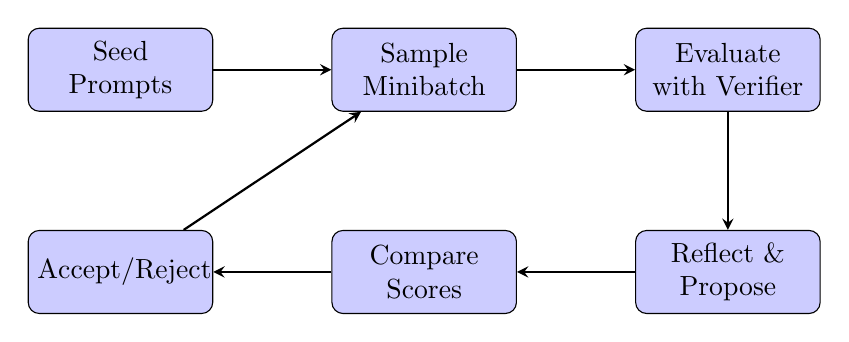
\begin{tikzpicture}[node distance=1.5cm, auto,
    block/.style={rectangle, draw, fill=blue!20, text width=6em, text centered, rounded corners, minimum height=3em},
    arrow/.style={->, >=stealth, thick}]
    
    \node[block] (seed) {Seed Prompts};
    \node[block, right=of seed] (sample) {Sample Minibatch};
    \node[block, right=of sample] (eval) {Evaluate with Verifier};
    \node[block, below=of eval] (reflect) {Reflect \& Propose};
    \node[block, left=of reflect] (compare) {Compare Scores};
    \node[block, left=of compare] (accept) {Accept/Reject};
    
    \draw[arrow] (seed) -- (sample);
    \draw[arrow] (sample) -- (eval);
    \draw[arrow] (eval) -- (reflect);
    \draw[arrow] (reflect) -- (compare);
    \draw[arrow] (compare) -- (accept);
    \draw[arrow] (accept) -- (sample);
\end{tikzpicture}
\caption{GEPA Optimization Loop}
\end{figure}

\subsection{Dataset}

\begin{itemize}
    \item \textbf{Source}: GSM8K mathematical reasoning benchmark
    \item \textbf{Training Set}: 2,074 low-confidence examples (verifier score $< 0.7$)
    \item \textbf{Validation Set}: 231 examples (10\% holdout)
    \item \textbf{Selection Criteria}: Only solutions requiring refinement were included
\end{itemize}

\subsection{Baseline Prompts}

The seed prompts used as the starting point:

\begin{lstlisting}[basicstyle=\small\ttfamily, frame=single, breaklines=true]
Critique Prompt:
"Review this solution step by step. Identify any errors 
in mathematical reasoning, calculations, or logic. 
Be specific about what went wrong."

Refinement Prompt:
"Based on the critique above, provide a corrected 
step-by-step solution. End your final answer with 
\boxed{answer}."
\end{lstlisting}

\section{Methodology}

\subsection{Scoring Function}

For each example, the score $s$ is computed based on correctness and improvement:

\begin{equation}
s = \begin{cases}
1.0 & \text{if refined solution is correct} \\
-0.5 & \text{if original correct} \land \text{refined incorrect (regression)} \\
0.5 \cdot \max(0, v_{\text{refined}} - v_{\text{original}}) & \text{otherwise (partial credit)}
\end{cases}
\end{equation}

where $v_{\text{original}}$ and $v_{\text{refined}}$ are verifier scores before and after refinement.

\subsection{GEPA Optimization Algorithm}

\begin{algorithm}
\caption{GEPA Prompt Optimization}
\begin{algorithmic}[1]
\State \textbf{Input:} Seed prompts $P_0$, training set $\mathcal{D}$, max iterations $T$
\State \textbf{Output:} Best prompts $P^*$
\State $P^* \gets P_0$; $s^* \gets \text{Evaluate}(P_0, \mathcal{D}_{\text{val}})$
\For{$t = 1$ to $T$}
    \State $c \gets t \mod 2$ \Comment{Alternate: critique or refinement}
    \State $\mathcal{M} \gets \text{SampleMinibatch}(\mathcal{D}_{\text{train}}, k=10)$
    \State $s_{\text{before}} \gets \text{Evaluate}(P_{\text{current}}, \mathcal{M})$
    \State $\mathcal{R} \gets \text{BuildReflectiveDataset}(P_{\text{current}}, \mathcal{M})$
    \State $P_{\text{new}}[c] \gets \text{ReflectAndPropose}(P_{\text{current}}[c], \mathcal{R})$
    \State $s_{\text{after}} \gets \text{Evaluate}(P_{\text{new}}, \mathcal{M})$
    \If{$s_{\text{after}} > s_{\text{before}}$}
        \State $s_{\text{val}} \gets \text{Evaluate}(P_{\text{new}}, \mathcal{D}_{\text{val}})$
        \State $P_{\text{current}} \gets P_{\text{new}}$
        \If{$s_{\text{val}} > s^*$}
            \State $P^* \gets P_{\text{new}}$; $s^* \gets s_{\text{val}}$
        \EndIf
    \EndIf
\EndFor
\State \Return $P^*$
\end{algorithmic}
\end{algorithm}

\subsection{Reflective Dataset Construction}

For each example in the minibatch, feedback is generated:

\begin{itemize}
    \item \textbf{SUCCESS}: ``Refinement corrected the answer to [ground\_truth]''
    \item \textbf{REGRESSION}: ``Original was correct but refinement made it incorrect''
    \item \textbf{PARTIAL}: ``Score improved by $\Delta v$ but still incorrect''
    \item \textbf{NO\_IMPROVEMENT}: ``Score decreased by $\Delta v$, correct answer was [ground\_truth]''
\end{itemize}

\section{Results}

\subsection{Optimization Trajectory}

\begin{table}[h]
\centering
\caption{Key Metrics Across 25 Iterations}
\begin{tabular}{lcc}
\toprule
\textbf{Metric} & \textbf{Value} \\
\midrule
Seed Validation Score & 0.1959 \\
Best Validation Score & 0.1979 \\
Absolute Improvement & +0.0019 \\
Relative Improvement & +0.98\% \\
Accepted Iterations & 10/25 (40\%) \\
Rejected Iterations & 15/25 (60\%) \\
\bottomrule
\end{tabular}
\end{table}

\subsection{Iteration-by-Iteration Analysis}

\begin{table}[h]
\centering
\caption{Minibatch Scores by Iteration (Selected)}
\begin{tabular}{cccccc}
\toprule
\textbf{Iter} & \textbf{Component} & \textbf{Before} & \textbf{After} & \textbf{Accepted} & \textbf{Best Val} \\
\midrule
1 & critique & 0.110 & 0.113 & Yes & 0.196 \\
2 & refinement & 0.100 & 0.141 & Yes & 0.196 \\
4 & refinement & 0.235 & 0.245 & Yes & 0.196 \\
9 & critique & 0.216 & 0.239 & Yes & 0.197 \\
18 & refinement & 0.100 & 0.119 & Yes & 0.198 \\
\bottomrule
\end{tabular}
\end{table}

\subsection{Score Distribution}

The validation scores across all 10 accepted candidates:

\begin{center}
\begin{tabular}{cc}
\toprule
\textbf{Candidate} & \textbf{Validation Score} \\
\midrule
1 (seed) & 0.1959 \\
2 & 0.1905 \\
3 & 0.1914 \\
4 & 0.1920 \\
5 & 0.1905 \\
6 & 0.1973 \\
7 & 0.1933 \\
8 (best) & \textbf{0.1979} \\
9 & 0.1954 \\
10 & 0.1888 \\
\bottomrule
\end{tabular}
\end{center}

\section{Analysis}

\subsection{Primary Finding: No Meaningful Prompt Evolution}

Despite 25 iterations and 10 accepted updates, the final evolved prompts are \textbf{identical to the seed prompts}. This indicates a fundamental failure in the reflection stage.

\subsection{Root Cause Analysis}

\subsubsection{1. Reflection Model Capacity}

Gemma 2-2B was used for both:
\begin{itemize}
    \item Executing the refinement task (generating critiques/solutions)
    \item Reflecting on execution traces to propose improvements
\end{itemize}

The reflection task requires higher-order reasoning that exceeds the model's capacity. GEPA's original implementation uses stronger models (GPT-4) for reflection.

\subsubsection{2. Prompt Extraction Failure}

The reflection output is parsed using regex:
\begin{lstlisting}[language=Python, basicstyle=\small\ttfamily]
match = re.search(r'```(?:\w*\n)?(.+?)```', response)
\end{lstlisting}

If the model doesn't format its output with code blocks, the extraction falls back to returning the original prompt unchanged.

\subsubsection{3. Feedback Granularity}

The reflective feedback provides only coarse signals:
\begin{itemize}
    \item ``SUCCESS'' or ``FAILURE'' labels
    \item Numeric score deltas
\end{itemize}

Finer-grained feedback (e.g., specific error patterns) would enable more targeted improvements.

\subsection{Why Scores Still Changed}

If prompts didn't change, why did validation scores vary (0.188 to 0.198)?

\begin{enumerate}
    \item \textbf{Stochastic Generation}: Temperature=0.7 in Gemma produces different outputs each run
    \item \textbf{Sampling Variance}: Different minibatch samples yield different scores
    \item \textbf{Validation Set Size}: 231 examples provides limited statistical stability
\end{enumerate}

\subsection{Interpretation of Scores}

A validation score of $\sim$0.2 means:
\begin{itemize}
    \item Approximately 20\% of refinements result in correct answers (score = 1.0)
    \item Or a combination of partial improvements and regressions averaging to 0.2
\end{itemize}

This represents the \textbf{baseline capability} of the self-correction system, not gains from optimization.

\section{Recommendations}

\subsection{Short-Term Fixes}

\begin{enumerate}
    \item \textbf{Use Stronger Reflection Model}: GPT-4 or Claude for the reflection stage:
    \begin{lstlisting}[language=Python, basicstyle=\small\ttfamily]
reflection_model = "gpt-4"  # via LiteLLM
    \end{lstlisting}
    
    \item \textbf{Add Logging}: Print raw reflection outputs to diagnose extraction:
    \begin{lstlisting}[language=Python, basicstyle=\small\ttfamily]
print(f"Raw reflection output:\n{response[:500]}")
    \end{lstlisting}
    
    \item \textbf{Increase Minibatch Size}: Use 25-30 examples for more stable signal.
\end{enumerate}

\subsection{Architectural Changes}

\begin{enumerate}
    \item \textbf{Few-Shot Reflection}: Include examples of prompt evolution in the meta-prompt
    \item \textbf{Richer Traces}: Include specific error types in feedback (arithmetic, logical, conceptual)
    \item \textbf{Separate Teacher Model}: Use a dedicated strong model for reflection only
\end{enumerate}

\section{Conclusion}

This experiment demonstrated a complete GEPA integration with a contrastive verifier system for mathematical self-correction. While the infrastructure functions correctly—producing valid scores, accepting/rejecting candidates, and saving results—the optimization achieved only marginal improvement (+0.98\%) due to the reflection model's inability to generate diverse, improved prompts.

The key insight is that \textbf{prompt optimization requires a model capable of meta-reasoning about prompt effectiveness}. Using the same 2B-parameter model for both execution and reflection is insufficient. Future work should employ a stronger reflection model (GPT-4 class) while maintaining the efficient Gemma model for execution.

\section{Appendix: Configuration}

\begin{lstlisting}[basicstyle=\small\ttfamily, frame=single]
{
  "max_iterations": 25,
  "minibatch_size": 10,
  "max_train_samples": -1,
  "score_threshold": 0.7,
  "verifier_checkpoint": "verifier_best.pt",
  "device": "cuda"
}
\end{lstlisting}

\end{document}
